\documentclass{article}
\usepackage{graphicx} % Required for inserting images

\title{Test OverleafSync}
\author{IWH Macro department}
\date{\today}

\begin{document}

\maketitle

\section{Introduction}

\begin{itemize} 
    \item A warm welcome to today's workshop!
    \item I hope to learn about Git and Overleaf with you!
    \item As you will see, both tools can be combined in a powerful way for collaborative writing!
    \item It is great to work with you
    \item I really look forward to work with you!
\end{itemize}

\section{Playgrounds}
In the following, everyone will be given the opportunity to add some words to their assigned paragraph in the local copy, and then push the changes to the common document.

\subsection{Playground 1: Katja}
GitHub, GitDesktop, GitBash - Pull and Push, Coffee and Tea
\\

\includegraphics[Test Figure]{Figures/Overleaf.PNG}
\\

new locally added figures:

\includegraphics[Test Figure]{Figures/Logo_IWH_English.PNG}

\subsection{Playground 2: Julian}
Thank you Erik and Macro department!

\subsection{Playground 3: Anna}
This workshop is very helpful for future collaborative works. Thank you for your work, Erik!
Now, I am doing a local change on this document.

\subsection{Playground 4: Oliver}
I don't like Mondays!
I have Friday on my mind.

\subsection{Playground 5: Andrej}
Overleaf is a collaborative LaTeX editor that simplifies writing and sharing scientific documents. By integrating Overleaf with GitHub, users can efficiently version control their LaTeX projects and collaborate seamlessly. This setup allows you to push changes from Overleaf to GitHub and pull updates from GitHub back into Overleaf. It ensures that document revisions are tracked, reducing the risk of errors in collaborative environments. Follow this guide to learn how to connect Overleaf with GitHub and manage your LaTeX documents effectively.

Overleaf est un éditeur collaboratif LaTeX qui simplifie la rédaction et le partage de documents scientifiques. En intégrant Overleaf avec GitHub, les utilisateurs peuvent gérer efficacement les versions de leurs projets LaTeX et collaborer en toute simplicité. Cette configuration permet de pousser les modifications d’Overleaf vers GitHub et de récupérer les mises à jour de GitHub dans Overleaf. Elle garantit que les révisions des documents sont suivies, réduisant ainsi le risque d’erreurs dans un environnement collaboratif. Suivez ce guide pour apprendre à connecter Overleaf à GitHub et gérer vos documents LaTeX de manière efficace.

\subsection{Playground 6: Hua}
It is quite useful. Thanks!
Now is sunny, wonderful.
Now is another trial

\subsection{Playground 7: Afroza}

\subsection{Playground 8: Mariia}

\subsection{Playground 9}
I understand now how overleaf works.
I aks ChatGPT what a locla clone is. I try chatgpt.
\subsection{Playground 10}




\section{Conflict provocation}
Conflicts may arise when working with colleagues on one common project. The following section contains five paragraphs, which the participants will be asked to change simultaneously in order to provoke conflicts!

\subsection{Conflict 1}
Macroeconomics forecasting is an awesome and beautiful discipline that helps us understand resource allocation and market operations. The IWH has significantly contributed through studies on the economic effects of structural change in Eastern Germany, offering valuable insights for similar regions.

\subsection{Conflict 2}
Economics informs public policy by analyzing data and developing models. IWH researchers have influenced policy debates on labor market reforms and fiscal federalism, but unfortunately nobody is really listening.

\subsection{Conflict 3}
Addressing global challenges like poverty and climate issues, economics offers evidence-based recommendations. 
Addressing global challenges like poverty and climate issues, economics offers evidence-based recommendations. The IWH's research on climate change economics suggests that thallphe benefits of sustainable development and the need for global cooperation.

\subsection{Conflict 4}
Economics is interdisciplinary, incorporating insights from psychology and sociology to understand human behavior. The IWH fosters collaboration between economists and other experts, leading to innovative research on social networks and cultural factors.

\subsection{Conflict 5}

Any main thing that is exposed to technological change, economics continually evolves to address new challenges. The IWH pioneers research on the digital economy and technological change, providing insights into taking advantage of digitalization benefits while mitigating risks.


% \newpage
% \section{A nice picture}
% \subsection{I try to add a figure}
% \begin{figure}[h]
%   \centering
%   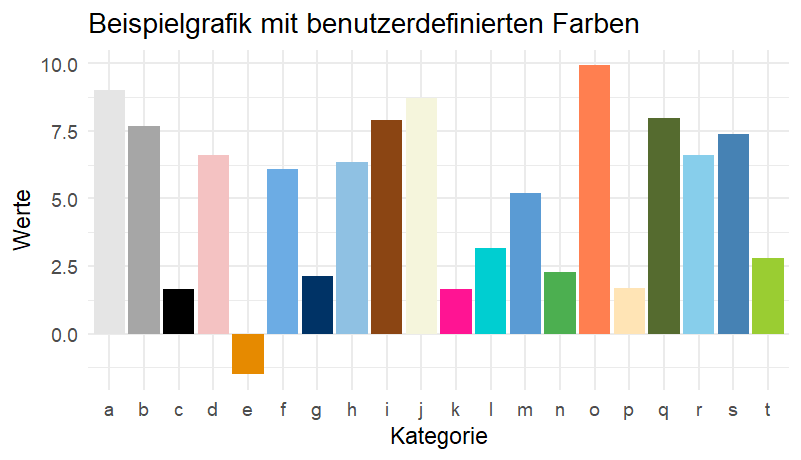
\includegraphics[width=\textwidth]{Figures/efn/plot_example.png}
%   \caption{Caption}
% \end{figure}

\end{document}
